\begingroup \color{OliveGreen}

\begin{figure}
\begin{center}
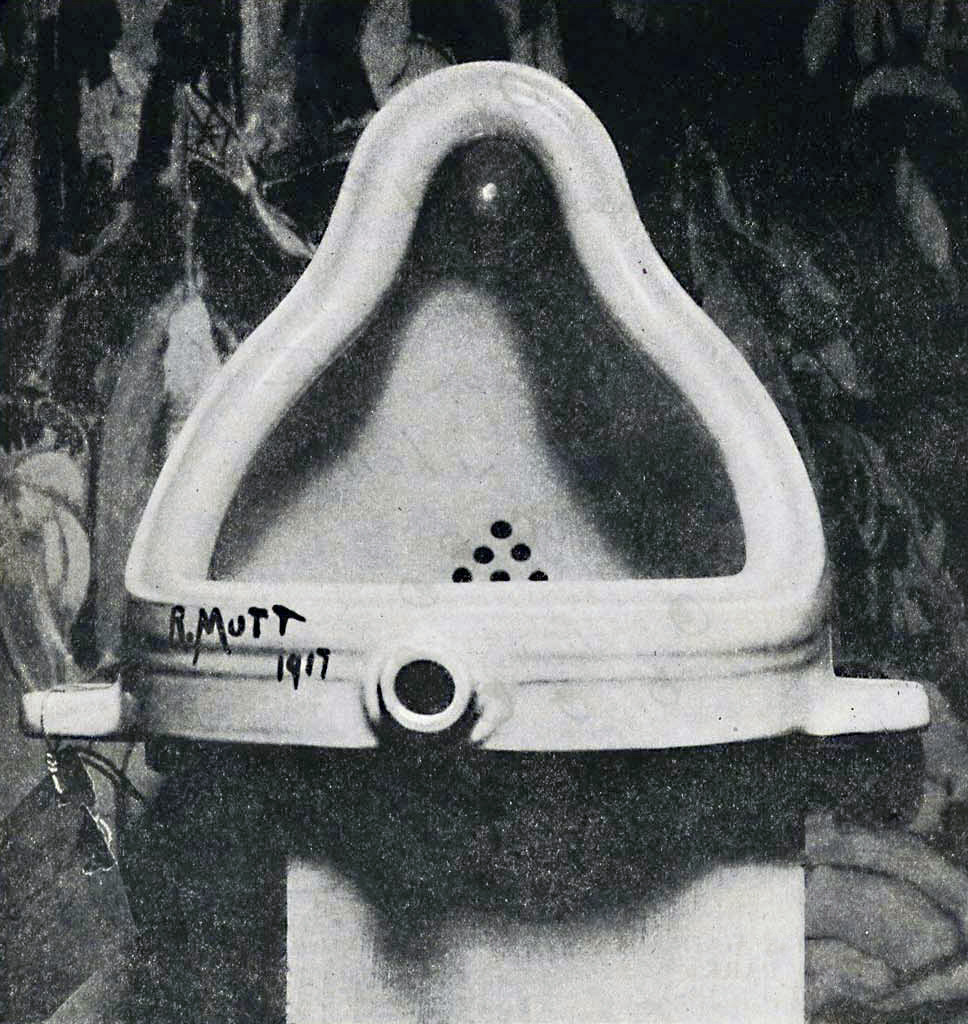
\includegraphics[width=.4\textwidth]{figures/Duchamp_Fountaine/Duchamp_Fountaine.jpg}
\end{center}
\caption{A paradigmatic example of found-art. Photograph by Alfred Stieglitz. Caption reads: ``Fountain by R. Mutt, Photograph by Alfred Stieglitz, THE EXHIBIT REFUSED BY THE INDEPENDENTS''. Public domain, via the Wikimedia Commons.}
\end{figure}

\section{Don't make what you can simply use, and don't sell what you can afford to give away} \label{sec:Use_or_make}
% DK: I am not sure about the [old] title of this pattern. The bulk of the body of the pattern seems to be about the reuse. Maybe something like “Don’t Make what you can Use” might fit the spirit better. [fixed]

\subsubsection*{Context}
% DK: This seems like an explanation of the title, not a context in which a problem is observed.
Peer production, as the name indicates, is about producing, in other words -- ``making stuff.''  Similarly, in academia, it's all about making an ``impact,'' and in business usually has something to do with making money.  But we only ever do any of this by building on the work of others.    

\subsubsection*{Problem}
People are often very attached to their own projects and priorities and don't have a sense of how their initiatives can benefit from connecting with others. Many projects die because the cost of \patternname{\href{http://c2.com/cgi/wiki?ReinventingTheWheel}{Reinventing the Wheel}} [c2] is too high.  We're often blind to the obstacles that we put in our own path.

\subsubsection*{Solution} Learning something new generally involves connecting deeply with what's already there.  While it's a great idea to ``steal like an artist'' don't forget to return the favor and make it possible for other people to remix and adapt your work too.  One good start is to give it away, then it's not technically stealing when others use it.
%\cite{anderson2009free}.
In our case, we've released the \emph{Peeragogy Handbook} using the Creative Commons Public Domain Dedication (CC0), a legal instrument grants the greatest possible leeway to downstream users.\footnote{\url{https://creativecommons.org/publicdomain/zero/1.0/}}  Show appreciation when someone takes up the offer.  (In the case of shared content, make backups so that you don't have to worry about losing the record of idea that another person might not have noticed was important.)

\subsubsection*{Rationale} 
Clearly we are not the first people to notice the problems with wheel-reinvention, including ``missing opportunities, repeating common mistakes, and working harder than we need to''\footnote{\url{https://blog.wikimedia.org/2013/11/19/learning-patterns-new-way-share-important-lessons/}}.  As Willow Brugh of Geeks without Bounds and the MIT Media Lab remarked as a guest in one of our hangouts\footnote{\url{https://www.youtube.com/watch?v=NpyQfYVKfBI}}: people often think that they need to build a community, and so fail to recognize that they are already part of a community.  Just as there can be subsequent benefits to helping your neighbor, it behooves us well to serve the communities that we are part of, rather than ignore them.   When we re-purpose the work of others, we potentially create a new bond.   When we think about how others can leapfrog ahead by building on our experiences, we prepare for something similar in the future.

\subsubsection*{Resolution}   It's worth keeping in mind that peeragogy per se is not new, and it's not something we can bottle and sell.  But we can try to learn how to do it more effectively.  Innovation doesn't come out of the blue -- and furthermore, as much as innovation is celebrated in our culture, there's something to be said for tradition, too.   The pattern \patternname{Don’t make what you can simply use, and don’t sell what you can afford to give away} is most useful because it shows how to make use of a shared language, or, if necessary, help build a one.  This is the best way to help get around those nasty self-placed obstacles.

\begin{framed}
\emph{What's Next.}
We've spun off the pattern catalog from the \emph{Peeragogy Handbook} into this paper, sharing it with a new community and gaining new perspectives.  Let's look for other parts of the handbook we can spin off!
\end{framed}

\endgroup
